%% %%%%%%%%%%%%%%%%%%%%%%%%%%%%%%%%%%%%%%%%%%%%%%%%
%% Problem Set/Assignment Template to be used by the
%% Food and Resource Economics Department - IFAS
%% University of Florida's graduates.
%% %%%%%%%%%%%%%%%%%%%%%%%%%%%%%%%%%%%%%%%%%%%%%%%%
%% Version 1.0 - November 2019
%% %%%%%%%%%%%%%%%%%%%%%%%%%%%%%%%%%%%%%%%%%%%%%%%%
%% Ariel Soto-Caro
%%  - asotocaro@ufl.edu
%%  - arielsotocaro@gmail.com
%% %%%%%%%%%%%%%%%%%%%%%%%%%%%%%%%%%%%%%%%%%%%%%%%%

\documentclass[12pt]{article}
\usepackage{design_ASC}
\usepackage{parskip}
\usepackage{listings}
\usepackage{longtable}
\usepackage{float}

\usepackage{titling}
\renewcommand\maketitlehooka{\null\mbox{}\vfill}
\renewcommand\maketitlehookd{\vfill\null}

\setlength\parindent{0pt} %% Do not touch this

%% -----------------------------
%% -----------------------------
%% %%%%%%%%%%%%%%%%%%%%%%%%%
\begin{document}
\setlength{\droptitle}{45mm}    
%% %%%%%%%%%%%%%%%%%%%%%%%%%
\begin{titlepage}
\begin{center}
\uppercase{
\textbf{Universidade de São Paulo}\\
\textsc{Escola de Engenharia de São Carlos}\\
\textsc{Instituto de Ciências Matemáticas e de Computação}
}
\hspace{5mm}\\[6cm]
\Huge{Projeto Prático II \\ Estimando a ordem via quadrados mínimos}\\[1cm]
\Large{SME0602 - Cálculo Numérico \\ Professor: Elias Salomão Helou Neto}\\[5cm]

\large{ 
\hspace*{\fill} Enrico Vicenzo Salvador Robazza\\ 
\hspace*{\fill} nº USP: 9806738\\[3cm]
29 de Julho de 2020
}
\end{center}
\end{titlepage}

% --------------------------
% Start here
% --------------------------

% %%%%%%%%%%%%%%%%%%%
\section*{Questão 1}
% %%%%%%%%%%%%%%%%%%%
Interpole a função\\[5pt]
$$
f(x) = \frac{1}{1+25x^2}
$$\\[10pt]
nos pontos $x_i = -1+2i/k$ com $i \in \{0,...,k\}$, por um polinômio. Denomine este interpolador $p_k$. \\
Calcule o valor de $e_k := max_{x \in [-1,1]}|f(x)-p_k(x)|$ e trace um gráfico de $e_k$ por $k$. Descreva o que você percebe. Este resultado contradiz o Teorema da Aproximação de Weierstrass? Explique. \\
\\
{\bfseries R:} Para a interpolação dos pontos, foram utilizados valores de $k \in \{2,...,100 \}$.
Primeiramente, é necessário encontrar os valores de $x_i$ com $i \in \{0,...,k \}$ para cada um dos $k$, então é interpolado o polinômio $p_k$ através do método de Lagrange, e calculado o erro máximo daquele polinômio no intervalo $[-1,1]$ com 200 pontos. Esses resultados são adicionados em uma lista de $e_k$'s. Por fim, a função retorna todos os $k$'s e $e_k$'s.\\

\begin{lstlisting}[language=Python]
def get_eks_lagrange(fx):
  eks = []
  ks = []
  for k in range(2, 100):
    x_nodes = get_x_nodes_for_k(k)
    y_nodes = fx(x_nodes)
    pk = lagrange(x_nodes, y_nodes)
    x_plot = np.linspace(-1,1,200)
    ek = max(np.absolute(fx(x_plot)-pk(x_plot)))
    ks.append(k)
    eks.append(ek)
  return (ks, eks)
\end{lstlisting}

Com isso, foi traçado o seguinte gráfico de $log(e_k)$ por $k$ referente aos erros máximos das interpolações:

\begin{figure}[H]
  \begin{center}
    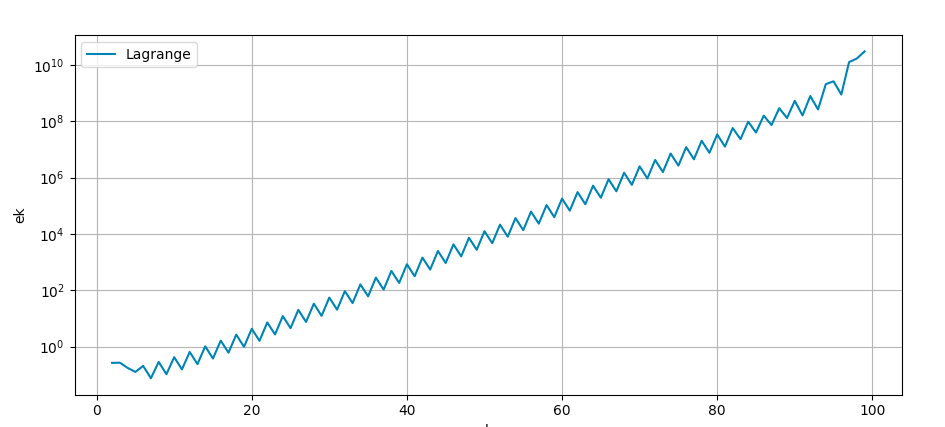
\includegraphics[width=0.8\linewidth]{lagrange_eks_semilogy.png}
  \end{center}
  \caption{Gráfico de log(ek) por k para Lagrange.}
  \label{fig:leastsquares1}
\end{figure}

Sobre estes resultados, podemos notar que $e_k \rightarrow \infty $ à medida que $k \rightarrow \infty $. Isso poderia indicar que o resultado contradiz o Teorema da Aproximação de Weirstrass, entretanto, o teorema não menciona nada a respeito dos pontos da interpolação, e se alterarmos os pontos utilizando os Nós de Chebyshev, de acordo com a equação:

$$
  x_i = \frac{a+b}{2} - \frac{b-a}{2} cos(\frac{k}{n} \pi),  \qquad \forall k = 0, 1, ... , n
$$
em que $a$ e $b$ é o intervalo da distribuição e $n$ é a quantidade de pontos, obtemos o seguinte resultado:

\begin{figure}[H]
  \begin{center}
    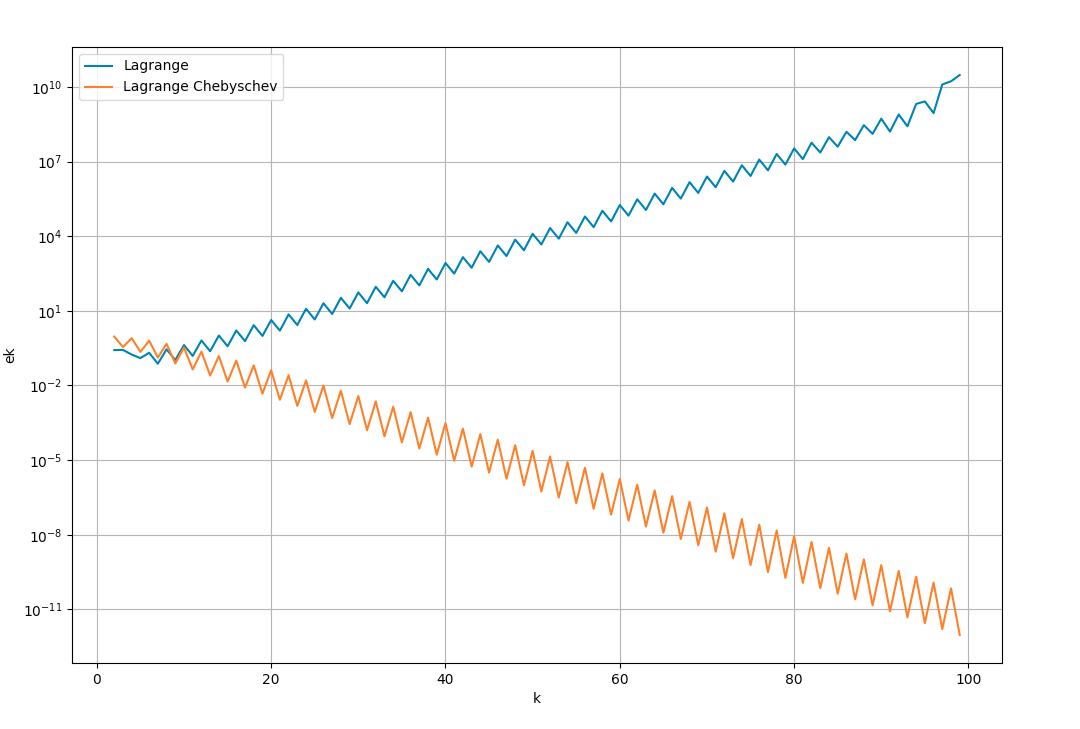
\includegraphics[width=0.8\linewidth]{lagrange_chebyshev.png}
  \end{center}
  \caption{Gráfico de log(ek) por k para Lagrange com nós de Chebyshev.}
  \label{fig:leastsquares1}
\end{figure}

Este fenómeno é conhecido como Fenómeno de Runge e ocorre quando os pontos de amostra são igualmente espaçados, o que é o caso da primeira interpolação.


% %%%%%%%%%%%%%%%%%%%
\section*{Questão 2}
% %%%%%%%%%%%%%%%%%%%
Interpole a mesma função da questão 1, nos mesmos pontos, agora utilizando \emph{splines} cúbicas naturais. \\
Avalie os resultados estudando a quantidade $max_{x \in [-1, 1]}|f(x) - s(x)|$ para cada um dos casos. Faça gráficos desses erros conforme aumenta o número de pontos de interpolação e interprete os resultados. Compare com os obtidos na questão 1.\\[10pt]
Supondo que o erro incorrido seja da forma $Ch^q$, onde $h$ é a distância entre dois sucessivos pontos de interpolação, estime q utilizando quadrados mínimos para o caso das splines naturais e para o caso da derivada conhecida nos extremos. \\[10pt]

{\bfseries R:} Para interpolar com splines cúbicas, foi utilizada uma função bem similiar a do método de Lagrange, em que a quantidade de pontos de interpolação varia em $k \in \{2,\;...\;,100\}$:
\\
\begin{lstlisting}[language=Python]
  def get_eks_spline(fx):
    eks = []
    ks = []
    for k in range(2, 100):
      x_nodes = get_x_nodes_for_k(k)
      y_nodes = fx(x_nodes)
      sk = CubicSpline(x_nodes, y_nodes, bc_type='natural')
      x_plot = np.linspace(-1,1,200)
      ek = max(np.absolute(fx(x_plot)-sk(x_plot)))
      ks.append(k)
      eks.append(ek)
    return (ks, eks)
\end{lstlisting}
Foi utilizada a implementação das Splines Cúbicas do pacote scipy, com o $bc\_type = "natural"$, o que significa que as derivadas de segunda ordem nas extremidades são iguais a 0. \\
Com a interpolação, foi traçado o seguinte gráfico de $log(e_k)$ por $k$:

\begin{figure}[H]
  \begin{center}
    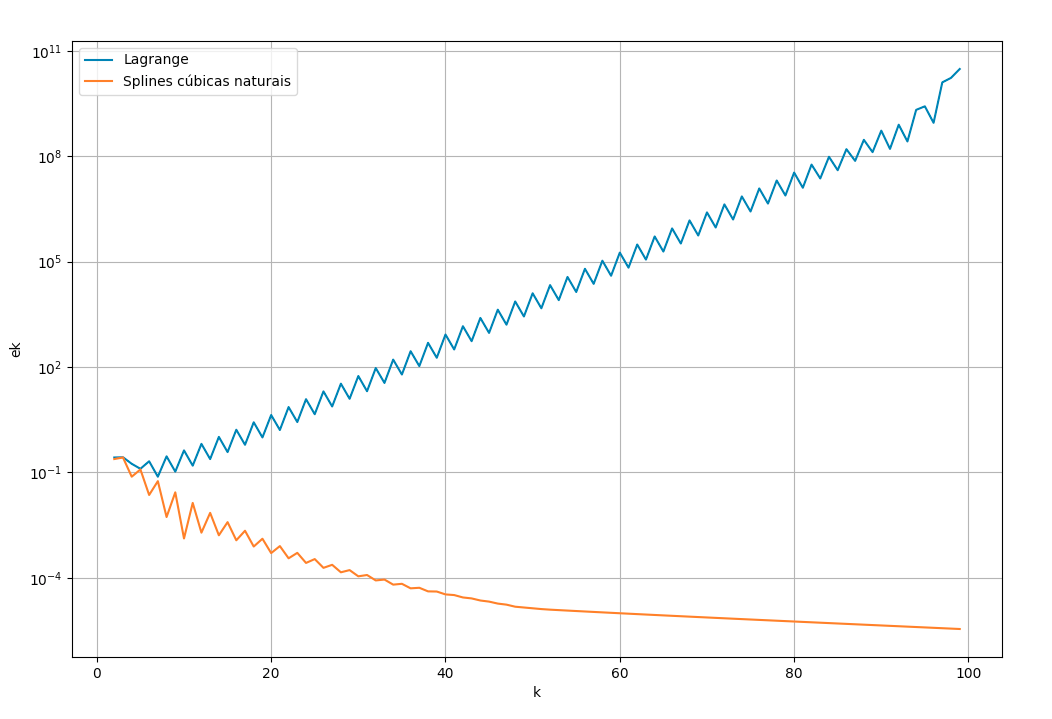
\includegraphics[width=0.8\linewidth]{splines_1.png}
  \end{center}
  \caption{Gráfico de log(ek) por k para Splines e Lagrange.}
  \label{fig:leastsquares1}
\end{figure}

De acordo com o gráfico, podemos notar que mesmo com os pontos igualmente espaçados, a medida que o número de pontos $k$ aumenta, $e_k$ diminui.\\
Podemos utilizar também a implementação das Splines Cúbicas com o caso das derivadas conhecidas nos extremos, uma vez que é possível calcular as derivadas da função. Para isso, foi utilizada a seguinte função:\\

\begin{lstlisting}[language=Python]
  def get_eks_spline_known_derivative(fx, fd2x):
    eks = []
    ks = []
    for k in range(2, 100):
      x_nodes = get_x_nodes_for_k(k)
      y_nodes = fx(x_nodes)
      dx1 = fd2x(x_nodes[0])
      dxn = fd2x(x_nodes[-1])
      sk = CubicSpline(x_nodes, y_nodes, bc_type=((2, dx1), (2, dxn)))
      x_plot = np.linspace(-1,1,200)
      ek = max(np.absolute(fx(x_plot)-sk(x_plot)))
      ks.append(k)
      eks.append(ek)
    return (ks, eks)
\end{lstlisting}

que recebe como parâmetros a função a ser interpolada e sua segunda derivada. Então, para cada $k$, são calculadas as derivadas nas extremidades, que por sua vez são utilizadas na interpolação por Splines Cúbicas. Com essa implementação, obtemos o seguinte gráfico de log(ek) por k:

\begin{figure}[H]
  \begin{center}
    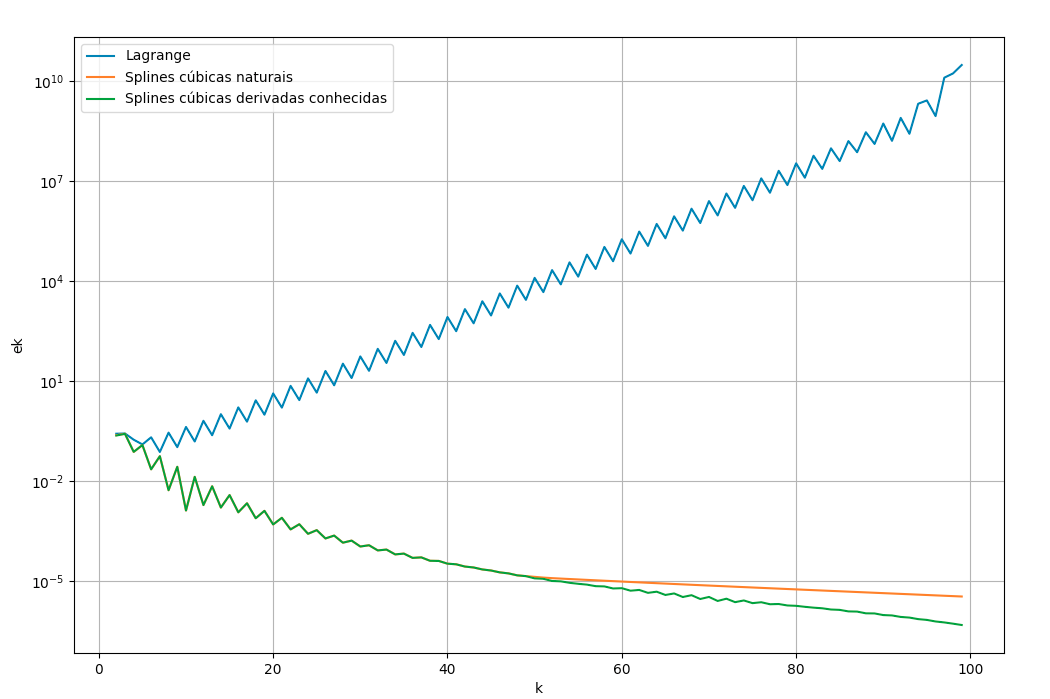
\includegraphics[width=0.8\linewidth]{splines_2.png}
  \end{center}
  \caption{Gráfico de log(ek) por k para Splines Naturais, Derivadas Conhecidas e Lagrange.}
  \label{fig:leastsquares1}
\end{figure}

Podemos analisar que os resultados obtidos são muito parecido às Splines Naturais, entretanto para um $k \geq 50$, $e_k$ passa a ser menor.\\

Supondo que o erro incorrido seja da forma $e(k) = Ck^q$, podemos linearizar essa função de forma que: 

\begin{align}
  \begin{split}
    log(e(k)) & = log(Ck^q) \\
    & = log(C) + q \; . \; log(k)
  \end{split}
\end{align}

Em que $q$ seria o coeficiente angular da reta, e $log(C)$ seria o coeficiente linear.\\
Se traçarmos um gráfico $log(e_k)$ por $log(k)$ tanto para as Splines Cúbicas Naturais quanto para a de derivadas conhecidas, obtemos:

\begin{figure}[H]
  \begin{center}
    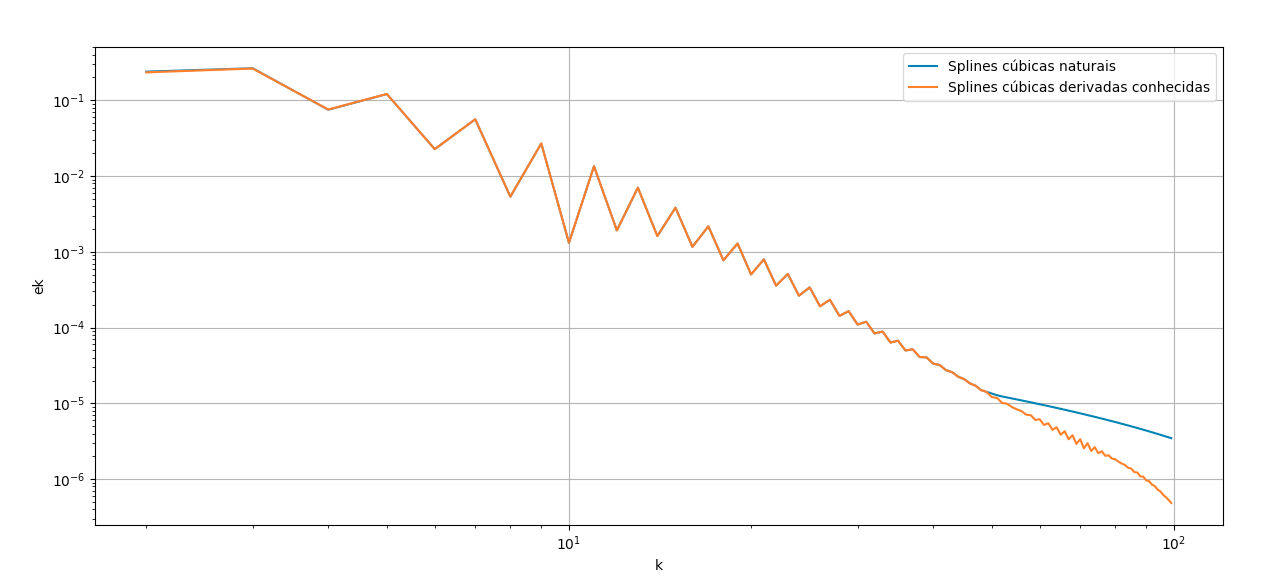
\includegraphics[width=0.8\linewidth]{loglog_1.png}
  \end{center}
  \caption{Gráfico de log(ek) por log(k) para Splines Naturais e Derivadas Conhecidas}
  \label{fig:leastsquares1}
\end{figure}

Com isso, podemos estimar o valor de q, através da interpolação dessa reta pelo Método dos Quadrados Mínimos, e então encontrar os coeficientes linear e angular:

\begin{lstlisting}[language=Python]
  k=2
  func = method.least_squares(np.log(ks2), np.log(eks2), k)
  x_plot = np.array(np.log(ks2))
  b = func(0)
  a = (func(x_plot[1])-b)/x_plot[1]
\end{lstlisting}

Em que $ks$ é o vetor com todos os $k \in \{ 2, \; ... \;, 100 \}$, $eks$ é o vetor contendo os erros, $b$ é o coeficiente linear e $a$ é o coeficiente angular.

Para a interpolação por Quadrados Mínimos, foi utilizada as seguintes funções:

\begin{lstlisting}[language=Python]
  def ft(t, x):
    soma = 0
    for i in range(len(x)):
      soma += x[i] * t ** i
    return soma

  def least_squares(x_nodes, y_nodes, k):
    A = np.empty((len(y_nodes), k))
    for i in range(len(y_nodes)):
      A[i] = [x_nodes[i] ** j for j in range(k)]
    AA = np.dot(A.T, A)
    Ab = np.dot(A.T, y_nodes)
    x = np.linalg.solve(AA, Ab)
    return lambda t: ft(t, x)
\end{lstlisting}

A função \emph{least\_squares} recebe como parâmetro os pontos de interpolação $(x, y)$, e um valor $k$ que é referente ao grau do polinômio a ser interpolado.

Com isso, é necessário encontrar 
$$ \underset{x \in \rm I\!R^n}{min} ||Ax-b||^2$$ 
resolvendo o sistema $A^T A = A^T b$, sendo que A é uma matriz $m \times k$ em que $m$ é a quantidade de pontos da amostra, como se segue:

$$
    \begin{bmatrix}
        x_1^0 & x_1^1 & x_1^2 & ... & x_1^k\\[10pt]
        x_2^0 & x_2^1 & x_2^2 & ... & x_2^k\\[10pt]
        & & .\\
        & & .\\
        & & .\\[10pt]
        x_m^0 & x_m^1 & x_m^2 & ... & x_m^k\\[10pt]
    \end{bmatrix}
$$

Encontrados os valores do vetor $x$, é retornada uma função $ft(t, x)$ que é a soma polinomial de todos os fatores.

Com isso, os resultados obtidos para as Splines Naturais foram:

\begin{figure}[H]
  \begin{center}
    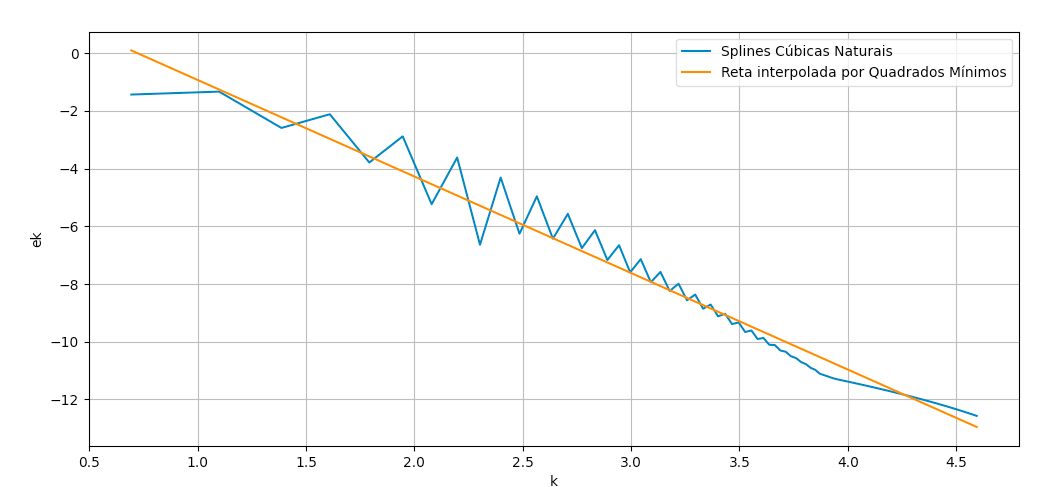
\includegraphics[width=0.8\linewidth]{splines_quadrados_minimos.png}
  \end{center}
  \caption{Interpolação por mínimos quadrados de ek para Splines Naturais}
  \label{fig:leastsquares1}
\end{figure}

A partir dessa função, conseguimos encontrar os valores de $a = -3.3459959287040517$ e $b = 2.41919397032667$.\\
Os resultados obtidos para as Splines com Derivadas Conhecidas foram:

\begin{figure}[H]
  \begin{center}
    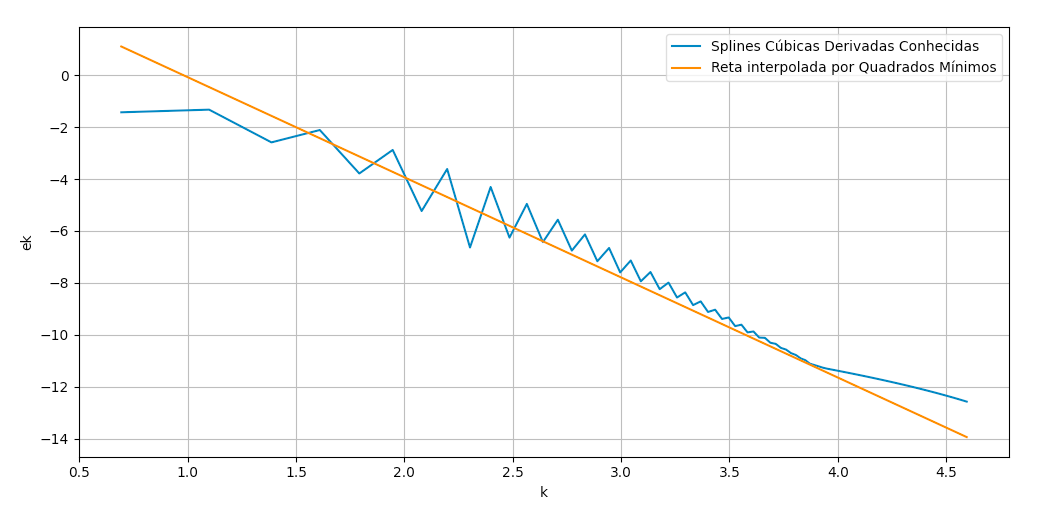
\includegraphics[width=0.8\linewidth]{splines_derivadas_quadrados.png}
  \end{center}
  \caption{Interpolação por mínimos quadrados de ek para Splines Derivadas Conhecidas}
  \label{fig:leastsquares1}
\end{figure}

A partir dessa função, conseguimos encontrar os valores de $a = -3.854345366863061$ e $b = 3.774497170458169$.\\
Com esses resultados, podemos chegar a conclusão de que o valor de $q$ para as Splines Cúbicas Naturais e para as Splines Cúbicas com Derivadas Conhecidas são, respectivamente, $-3.3459959287040517$ e $-3.854345366863061$, e portanto, a segunda tem uma ordem de convergência maior do que a primeira.

\end{document}